\documentclass[11pt,]{article}
\usepackage{lmodern}
\usepackage{amssymb,amsmath}
\usepackage{ifxetex,ifluatex}
\usepackage{fixltx2e} % provides \textsubscript
\ifnum 0\ifxetex 1\fi\ifluatex 1\fi=0 % if pdftex
  \usepackage[T1]{fontenc}
  \usepackage[utf8]{inputenc}
\else % if luatex or xelatex
  \ifxetex
    \usepackage{mathspec}
  \else
    \usepackage{fontspec}
  \fi
  \defaultfontfeatures{Ligatures=TeX,Scale=MatchLowercase}
\fi
% use upquote if available, for straight quotes in verbatim environments
\IfFileExists{upquote.sty}{\usepackage{upquote}}{}
% use microtype if available
\IfFileExists{microtype.sty}{%
\usepackage{microtype}
\UseMicrotypeSet[protrusion]{basicmath} % disable protrusion for tt fonts
}{}
\usepackage[margin=1.0in]{geometry}
\usepackage{hyperref}
\hypersetup{unicode=true,
            pdftitle={The fecal microbiome as a tool for monitoring and predicting response outcomes in Ustekinumab-treated, anti-TNF-alpha refractory Crohn's Disease patients.},
            pdfborder={0 0 0},
            breaklinks=true}
\urlstyle{same}  % don't use monospace font for urls
\usepackage{graphicx,grffile}
\makeatletter
\def\maxwidth{\ifdim\Gin@nat@width>\linewidth\linewidth\else\Gin@nat@width\fi}
\def\maxheight{\ifdim\Gin@nat@height>\textheight\textheight\else\Gin@nat@height\fi}
\makeatother
% Scale images if necessary, so that they will not overflow the page
% margins by default, and it is still possible to overwrite the defaults
% using explicit options in \includegraphics[width, height, ...]{}
\setkeys{Gin}{width=\maxwidth,height=\maxheight,keepaspectratio}
\IfFileExists{parskip.sty}{%
\usepackage{parskip}
}{% else
\setlength{\parindent}{0pt}
\setlength{\parskip}{6pt plus 2pt minus 1pt}
}
\setlength{\emergencystretch}{3em}  % prevent overfull lines
\providecommand{\tightlist}{%
  \setlength{\itemsep}{0pt}\setlength{\parskip}{0pt}}
\setcounter{secnumdepth}{0}
% Redefines (sub)paragraphs to behave more like sections
\ifx\paragraph\undefined\else
\let\oldparagraph\paragraph
\renewcommand{\paragraph}[1]{\oldparagraph{#1}\mbox{}}
\fi
\ifx\subparagraph\undefined\else
\let\oldsubparagraph\subparagraph
\renewcommand{\subparagraph}[1]{\oldsubparagraph{#1}\mbox{}}
\fi

%%% Use protect on footnotes to avoid problems with footnotes in titles
\let\rmarkdownfootnote\footnote%
\def\footnote{\protect\rmarkdownfootnote}

%%% Change title format to be more compact
\usepackage{titling}

% Create subtitle command for use in maketitle
\newcommand{\subtitle}[1]{
  \posttitle{
    \begin{center}\large#1\end{center}
    }
}

\setlength{\droptitle}{-2em}
  \title{The fecal microbiome as a tool for monitoring and predicting response
outcomes in Ustekinumab-treated, anti-TNF-alpha refractory Crohn's
Disease patients.}
  \pretitle{\vspace{\droptitle}\centering\huge}
  \posttitle{\par}
  \author{}
  \preauthor{}\postauthor{}
  \date{}
  \predate{}\postdate{}

\usepackage{setspace}
\doublespacing
\usepackage{lineno}
\linenumbers
\renewcommand{\familydefault}{\sfdefault}

\begin{document}
\maketitle

\vspace{35mm}

Running title: The fecal microbiome as a tool for monitoring and
predicting response outcomes in Ustekinumab-treated, anti-TNF-alpha
refractory Crohn's Disease patients.

\vspace{35mm} Matthew K. Doherty\({^2}\), Tao Ding\({^2}\)\({^\alpha}\),
Charlie Koumpouras\({^2}\), Shannon Telesco\({^1}\), Calixte
Monast\({^1}\), and Patrick D. Schloss\({^2}\)\({^\dagger}\)

\(\dagger\) To whom correspondence should be addressed:
\href{mailto:pschloss@umich.edu}{\nolinkurl{pschloss@umich.edu}}

1. Janssen Pharmaceutical Companies of Johnson \({\&}\) Johnson, Spring
House, PA, USA

2. Department of Microbiology and Immunology, University of Michigan,
Ann Arbor, MI, USA

\({\alpha}\) Currently at \emph{\ldots{}}

\newpage

\subsection{Abstract}\label{abstract}

\emph{Background:} Crohn's disease (CD) is a global health issue
characterized by patches of ulceration and inflammation along the
gastrointestinal tract. Individuals with CD have reduced microbial
diversity in their guts, compared to healthy individuals. It remains
unclear if this reduced diversity is a result or cause of pathogenesis.
We investigated the relationship between the fecal microbiome and
clinical phenotypes in subjects with moderate to severe CD treated with
Ustekinumab (UST) in a Phase 2b study to determine whether the fecal
microbiome at baseline is predictive of disease severity and therapeutic
response, as well as if the fecal microbiota changes due to therapy.

\emph{Methods:} The 16S rRNA gene from patient stool samples was
sequenced using the Illumina MiSeq platform. The resulting sequences
were curated and assigned to taxonomic groups using the mothur software
package to determine the bacterial communities and relative abundance of
bacterial species present in these patients. The relative abundance
among the fecal microbiota, patient demographic data, and clinical
metadata were used as input to a random forest machine-learning
algorithm to predict disease severity and response to treatment with
UST.

\emph{Results:} Fecal microbial diversity at baseline significantly
correlates with markers for disease severity, such as Crohn's Disease
Activity Index (CDAI), stool frequency, and disease duration.
Additionally, the overall community structure of the microbiome was
significantly different based on stool frequency, CRP, fecal
lactoferrin, fecal calprotectin, corticosteroid use, disease duration,
and tissue involvement. Baseline fecal microbiome community structures
and species diversity were significantly different among responders and
non-responders to UST treatment. Faecalibacterium, among other taxa, was
significantly more abundant in responders/remitters. Additionally, the
microbiome of clinical responders changed over time, in contrast to
nonresponsive subjects. Using AUC-RF, differences in the baseline
microbiome and clinical metadata were able to predict response to UST,
especially remission, with some AUCs approaching 0.85.

\emph{Conclusions:} The ability to predict and monitor response to
treatment using the microbiome will likely provide another clinical tool
in treating CD patients. Additionally, the observed baseline differences
in fecal microbiota and changes due to therapeutic response will allow
further investigation into the microbes important in CD pathogenesis as
well as establishing and maintaining CD remission. Finally, beneficial
microbes associated with response to treatment could be developed as
probiotics to increase the likelihood of response while undergoing
treatment.

\textbf{Keywords: Crohn's Disease, fecal microbiome, biologics,
prediction}

\newpage

\subsubsection{Introduction}\label{introduction}

Crohn's disease (CD), an incurable inflammatory bowel disease (IBD), is
a global health issue with increasing incidence. CD affects
approximately 3 million people worldwide, causing large economic and
healthcare utilization impacts on society (1--3). CD is characterized by
patches of ulceration and inflammation affecting the entire bowel wall
along the gastrointestinal tract, most commonly in the ileum and colon.
Individuals with CD experience frequent diarrhea, abdominal pain,
fatigue, and weight loss resulting in significant health care costs,
lower quality of life, and economic impacts due to loss of productivity
({\textbf{???}}, 2, 4) (2, 4, 5). Current treatments for CD include
antibiotics, anti-inflammatory drugs, immunomodulators, surgery, and
biologic agents targeting tumor necrosis factor alpha
(TNF-\({\alpha}\)), such as Infliximab (Remicade). Within 10 years of
diagnosis, approximately half of individuals with CD will require
surgery and the majority will experience escalating immunosuppressive
treatment (5) (6). Currently, individuals with CD are treated based on
disease location and risk of complications using escalating
immunosuppressive treatment and/or surgery with the goal of achieving
and sustaining remission (4, 6) (5, 7). Faster induction of remission
following diagnosis reduces the risk of irreversible intestinal damage
and disability (6--8) (7-9). Anti-TNF-\({\alpha}\) therapy in
combination with thiopurines has emerged as the preferred treatment for
CD, but up to half of individuals with CD fail to respond or lose
response to anti-TNF-\({\alpha}\) therapy (5, 6) (6, 7). Ustekinumab
(UST), a monoclonal antibody directed against the shared p40 subunit of
IL-12 and IL-23, has been proposed as an alternative therapy for these
patients (9) (10). While clinical trials have demonstrated that UST is a
viable option for the treatment of CD (6, 9--11) (7, 10-12), some
patients within these trials were non-responsive to UST, which may be
explained by differences in the patients' gut microbiomes.

The precise etiology of CD remains unknown, but host genetics,
environmental exposure, and the gut microbiome appear involved (1, 13).
Genome-wide association studies of individuals with CD identified
several susceptibility genes including NOD2, a receptor involved in
bacterial killing and innate immunity. Defects in NOD2 function affects
microbial sensing, the regulation of IL-23 driven Th17 responses, and
indirect modulation of the gut microbiome (5, 14). The gut microbiome
has also been shown to play a key role in inflammation, immunity, and
IBD (15). Individuals with CD have reduced microbial diversity in their
guts, compared to healthy individuals, with a lower relative abundance
of Firmicutes and an increased relative abundance of Enterobacteraciae
and Bacteroides, at the phylum level (14, 16-19). Additionally, previous
studies have shown that the gut microbiome can be predictive of disease
severity in new-onset, pediatric CD patients (19, 20). It remains to be
determined, however, whether the microbiome can predict response to
therapy in CD (14). Additionally, the effect of biologic treatment on
the gut microbiome is not well understood. If the fecal microbiome can
be used as a theraprognostic tool to non-invasively determine and
monitor disease severity as well as predict response to specific
treatment modalities, then more targeted treatment could result in
reduced adverse effects of less effective therapies and faster
achievement of remission.

Our lab was approached to analyze the gut microbiomes of individuals who
participated in a Phase II clinical trial to determine the efficacy of
UST in treating CD (10). Using stool samples taken prior to the start of
the study, 16S rRNA gene sequence data from these patients will allow us
to determine associations between clinical metadata, disease severity,
and the fecal microbiome and whether clinical responders have a
microbiome that is distinct from non-responders at baseline. Preliminary
results generated with fecal samples from a subset of study participants
and sequenced using the Roche 454 platform suggest that the fecal
microbiota of moderate to severe CD patients refractory to
anti-TNF-\({\alpha}\) may differentiate individuals who will respond to
treatment with UST; however, large interpersonal variation limited the
power of our findings. This study attempts to overcome many of the
limitations in our preliminary analysis by increasing our sample size to
the full patient cohort and using the Illumina MiSeq platform to improve
our sequencing depth. We demonstrate that the fecal microbiome is
associated with baseline clinical metadata and that these associations
and differences are useful in predicting disease severity and treatment
outcome.

\subsection{Results}\label{results}

\textbf{Characteristics of Study Population} We studied the fecal
microbiota in a subset of TNF-\({\alpha}\) refractory CD patients who
took park in the CERTIFI clinical trial described in Sandborn et al 2012
(10). Briefly, patients with a history of moderate to severe CD were
randomly assigned to a treatment group in the induction phase of the
study. Subjects provided a stool sample at screening (Week 0), Week 4
and Week 6. At Week 8 patients were re-randomized into maintenance
therapy groups. A final stool sample was provided at Week 22. Response
to therapy was evaluated at week 4, 6, 8, and 22 based on change in
CDAI. Samples from subjects that completed the clinical trial and had
complete clinical metadata were included in our analysis. We used 16s
rRNA gene sequencing to analyze the microbiome from 306 fecal samples
provided prior to treatment as well as 258 Week 4, 289 Week 6, and 205
Week 22 post-treatment fecal samples, for a total of 1058 samples.
Demographic and baseline disease characteristics are summarized in
supplemental table 1.

\textbf{Comparison of microbiome at screening based on clinical
variables} To determine if there were any significant associations
between microbial diversity and clinical variables of interest, we
compared the microbiome with clinical data at Week 0. We determined
species richness (\({\alpha}\)-diversity) using the inverse Simpson
metric and assessed associations between species richness and clinical
data using Spearman's rank correlation, Wilcoxon rank-sum, or
Kruskal-Wallis rank-sum tests. Associations between the overall
community structure (ß-diversity) and clinical data were determined
using the thetaYC distance metric as input to the adonis PERMANOVA
function within the vegan R package (21). As seen in table 1, we
observed a correlation between CDAI and species richness, with higher
CDAI correlating to lower richness. The overall community structure was
not different based on CDAI. When looking at CDAI subscores, we observed
a significant association between species richness and the frequency of
loose stools per week. The overall community structure was also
significantly different based on weekly loose stool frequency. No
significant association was observed between CRP and fecal calprotectin
and species richness, while higher fecal lactoferrin weakly correlates
with higher richness. The overall community structure was significantly
different based on CRP, fecal calprotectin, and fecal lactoferrin. No
significant differences in the microbiome were observed for BMI, weight,
or sex. Overall community structure was different based on age. The
overall community structure was also different based on the tissue
affected. Species richness and the overall community structure were
significantly different based on corticosteroid use. The community
structure was significantly different based on disease duration and a
significant correlation was seen between species richness and disease
duration, with lower richness corresponding to longer disease.

\emph{consider including LEfSe data for quick look at discriminate OTU
based on sig dif clinical variables like in Gevers and Zackular papers?}

\textbf{Comparison of clinical responders and non-responders} Next, We
wanted to see if there were associations between the microbiome at
baseline and response to treatment. For this study, response was defined
as a 30\% decrease from CDAI at baseline and remission defined as a CDAI
below 150. Of the 306 screening samples analyzed, 232 were from subjects
receiving UST and 74 from subjects receiving placebo. Baseline fecal
microbiome community structures and species diversity were different
among responders and non-responders to UST treatment. Based on response
at the primary endpoint of the study, 6 weeks after IV induction, there
was no difference in species richness between response groups, but there
was a significant difference in the overall community structure of the
entire cohort. This difference in community structure was not
significant in treatment vs.~placebo groups. Week 6 remitters were
significantly different from non-remitters in both species richness
(0.0005) and overall community structure (0.017). When looking at
treated vs.~untreated Week 6 remitters, the treated group had
significant differences in both species richness and community structure
while untreated remitters we not different from untreated non-remitters.
At the secondary endpoint, 22 weeks after IV-induction and 14 weeks
after maintenance dosing, there was no difference in species richness
between response groups, but there was a significant difference in the
overall community structure of the entire cohort. Week 22 remitters were
significantly different from non-remitters in both species richness
(0.57) and overall community structure (0.016). However, these
differences were not seen when the cohort was broken down by induction
group. This could be due to changes in maintenance treatment.

\textbf{The microbiome by treatment and response over time} One major
question with regards to biologic treatment of IBD and the microbiome is
whether treatment has an effect on the microbiome. We explored this
question 2 different ways. We included subjects that had stool samples
at all 4 time points and another analysis using subjects who provided
samples at weeks 0, 4, and 6. We used PERMANOVA stratified on each
subject, as a proxy for a repeated measures ANOVA, to determine if the
microbiome changed over time. We found that taken together treatment
does not affect the microbiome. No significant difference was seen based
on visit when looking at all groups and response status at week 4, 6, or
8 over the first 3 time points, but there was a significant interaction
between response at week 22 and visit (p=0.001) and between relative
response, induction group, and visit (p=0.0445).

This led us to examining just the week 22 responders vs.~non-responders
across visit. No significant difference over time was observed in
non-responders. When we segregated week 22 responders, we saw a
significant change in community structure over time. There was also a
significant difference based on treatment group, but no significant
interaction. When looking at treated vs.~untreated responder groups, we
observed a significant difference based on visit in the treated, Week 22
responder and in untreated responders across the first 3 visits prior to
maintenance phase.

When looking at time in all subjects across all 4 time points we
observed a significant interaction between visit and response, however
no interaction between visit, treatment group, and response. In all
subjects there was a significant difference in community structure based
on response at Week 22. In treated subjects, we observed a significant
interaction between response and visit, as well as a significant
difference in community structure based on response at Week 22. No
significant difference was observed in untreated responders across all 4
time points.

\textbf{Prediction of response based on the microbiome at screening}

Another major question in IBD and the microbiome is if response can be
predicted using the microbiome. To address this we used AUCRF to develop
a random forest classification model to differentiate responders from
non-responders, as well as remitters from non-remitters, based on the
relative abundance of fecal microbiome community members, clinical
metadata, and combined microbiome and clinical data (22, 23). We ran
these models for response and remission at Week 4, 6, 8, and 22 of the
study. The optimal models for response and remission at the primary
endpoint (Week 6) are shown in Figure 1. Using only clinical metadata to
predict response, the model predicted response with an AUC of 0.662 with
a specificity of 0.807 and a sensitivity of 0.524. Using only microbiome
data, the model predicted response with an AUC of 0.737 with a
specificity of 0.753 and a sensitivity of 0.622. When combining clinical
metadata with the microbiome, the model predicted response with an AUC
of 0.742 with a specificity of 0.787 and a sensitivity of 0.622. With
respect to Week 6 remission, using solely clinical metadata we achieved
AUC of 0.625 with a specificity of 0.711 and a sensitivity of 0.581.
Using only fecal microbiome data we achieved an AUC of 0.837 with a
specificity of 0.716 and a sensitivity of 0.903. When combining clinical
metadata with the microbiome AUC of 0.818 with a specificity of 0.721
and a sensitivity of 0.839.

Across all weeks and responses, prediction with clinical metadata alone
did not perform as well as models using the fecal microbiome at
screening. Also, combining microbiome data with clinical metadata did
not consistently improve prediction compared to microbiome data alone.
Additionally we found several OTUs occurred frequently across models
including Faecalibacterium, among other taxa that were significantly
more abundant in responders/remitters. Their abundances can be seen in
figure 4.

In addition to predicting future response, we wanted to determine if the
microbiome could be used to monitor response to therapy. Again we used
AUC-RF in order to determine if the fecal microbiome at Week 6 could be
used to determine response or remission at Week 6. As seen in
Supplemental Figure 1, using the microbiome alone we achieved an AUC of
0.696 for response with a sensitivity of 0.641 and a specificity of
0.711. For remission we had an AUC of 0.838 with a sensitivity of 0.767
and specificity of 0.816. Again we were better able to distinguish
remitters from non-remitters than responders/non-responders. The
clinical data were more reliable for determining disease activity at
Week 6.

\subsection{Discussion}\label{discussion}

Our results examine the fecal microbiome of a subset of patients who
participated in the CERTIFI trials to determine if the microbiome can
predict response to therapy and if therapy has any effect on the
microbiome. Several previous studies have looked at fecal and mucosal
microbiomes in pediatric patients with new-onset and established disease
and with established disease in adults (19, 24, 25). Unlike these
studies, our patients were mostly Caucasian adults in their late
thirties to early forties who failed to respond or lost response to
anti-TNF-\({\alpha}\) biologic treatment. We were able to find
associations between the fecal microbiome of these patients and CDAI,
stool frequency, fecal calprotectin, fecal lactoferrin, serum CRP,
corticosteroid use, tissue involvement, and duration of disease.

The association of the microbiome with clinically relevant biomarkers
and disease activity metrics indicates that the microbiome may also
function as a biomarker for CD activity. Given that serum CRP,
calprotectin, and lactoferrin are used as biomarkers to measure
intestinal inflammation and CD severity, it is interesting to see that
the microbial community structure is different among patients based on
these markers (26, 27). This supports the idea that the microbiome could
be useful as a biomarker for measuring disease activity in patients,
especially when considered in relation to these biomarkers (25). Higher
CDAI was associated with lower microbial diversity. This appears to be
consistent with other studies on the microbiome in individuals with CD
compared to healthy individuals and studies looking at active disease
compared to remission (19, 24, 25). However, these differences may have
been driven by weekly stool frequency, one component of the CDAI, where
higher stool frequency is also negatively associated with microbial
diversity. Given that higher stool frequency is associated with looser
stool consistency, this finding appears consistent with the association
between loose stools and lower diversity (28).

We also observed differences in the microbiome in relation to other
clinical variables. The microbial community structure was different
based on disease localization. These results are consistent with a study
by Naftali et al finding distinct microbiotas for ileal versus colonic
CD using mucosal tissue (29). This study also found that corticosteroid
use impacts the composition of the human fecal microbiome. This supports
data seen in the mouse model where corticosteroid injections altered the
fecal mouse microbiome (30). As corticosteroid use appears to impact
diversity, corticosteroids may be useful when trying to positively
impact the microbiome during biologic therapy and increase the
possibility of response to CD therapies.

Unlike other studies, these patients had a CD diagnosis for an average
of 12 years (Supplemental Table 1) (19, 24, 25). We observed that that
longer disease duration is associated with a reduction in fecal
microbial diversity. This decreased diversity may be due to the long
duration of inflammatory conditions in the gut. One could hypothesize
earlier biologic intervention may `preserve' microbiome that promotes
remission and reduces the likelihood of relapse. Publications have come
out in support of earlier biologic intervention, as it appears to
increase the likelihood of inducing remission and mucosal healing
(31-33). However, the cost of biologics for patients is hindrance to
early biologic intervention. Using aptamers in place of monoclonal
antibodies may reduce this cost and make earlier intervention possible.
Aptamers are short strands of DNA or RNA capable of specifically binding
small molecules, proteins, and whole cells. Anti-TNF aptamers have been
published that could potentially be used to test this in the mouse model
(34).

One important question for the microbiome and IBD is whether or not the
microbiome is affected by treatment with biologics. This study attempted
to answer that question by looking at the microbiome of our CD subjects
across multiple time points during treatment. While we were unable to
see direct effects of the drug on the fecal microbiome, we observed that
the microbiome of clinical responders changed over time, in contrast to
nonresponsive subjects. This was observed for responsive patients
regardless of induction treatment, leading us to think we are seeing the
effects of change in disease activity and health rather than any effects
from treatment. This interpretation is consistent with studies using the
microbiome to distinguish between remission and active CD (25). We did
however observe a significant difference in community structure based on
treatment and cannot eliminate the possibility of a direct effect on the
microbiome in treated responders.

Another important question in for the importance of the microbiome in
IBD is whether response to therapy can be predicted with the microbiome.
We attempted to address this by developing a random-forest model that
used relative microbial abundance data and/or clinical metadata for
input. We found we were better able to predict remission status compared
to response status. Response may be less predictable due to the
``floating target'' nature of a relative decrease in CDAI compared to
the hard threshold for remission (CDAI\textless{}150). We were also
better able to distinguish remission/non-remission than
response/non-response, 6 weeks after beginning treatment. This is
consistent with other studies again suggesting the microbiome could be
useful in detecting remission versus active disease (25).

While using the presented model may not be useful clinically to predict
response to therapy at this time, it is useful for hypothesis generation
about the biology of CD as it relates to the microbiome. Some of the
frequently occurring factors in our predictive models have already been
linked to CD pathogenesis. As far as clinical biomarkers, fecal
lactoferrin and fecal calprotectin occurred in the majority of models
where clinical metadata was combined with the microbiome, supporting
their importance as biomarkers for CD activity, especially in relation
tot eh fecal microbiome (26, 27). Faecalibacterium was the most
frequently occurring OTU in our models. It is associated with health and
has been shown to be low in CD patients (14, 17, 29, 35). Remission was
much more likely in individuals who had measurable Faecalibacterium
present at baseline. This supports the hypothesis that Faecalibacterium
impacts CD. Escherichia/Shigella also occurred frequently in our models.
This OTU is associated with inflammation and has been shown to
negatively impact CD (35). Fusobacterium also appeared in our predictive
models and is associated with CD and CRC, something CD patients are more
likely to get (35). These observations and the positive/negative
associations of these microbes and CD allow us to hypothesize on ways to
alter the microbiome to increase the likelihood therapeutic response.
Prior to the initiation of therapy, patients could get a fecal
microbiome analysis. The community data could then be used to direct the
patient to undergo a round of antibiotics to target and reduce the
levels of Escherichia in the patient's gut. Alternatively, the microbes
found to be positively associated with response could be formulated into
a daily probiotic patients could take while receiving therapy with the
goal of increasing the likelihood of remission and mucosal healing.

With this study we sought to gain a more detailed understanding of if
and how biologic treatment affects the microbiome, to determine whether
the microbiome can be used to identify patients who will respond to
therapy, and to gain a better understanding of the interaction between
the human gut microbiome and CD pathogenesis in adult patients. We found
the fecal microbiome to be useful in uncovering associations between the
microbiome and aspects of CD severity metrics and treatment outcomes. We
also demonstrated that the microbiome of treated responders changed over
time, though it is not yet possible to determine any direct effect of
treatment on the microbiome. Finally, we were able to show that the
microbiome could be useful in predicting response to therapy, especially
clinical remission, compared to clinical metadata alone in our unique
patient cohort. While this prediction is not clinically useful as of
yet, altering the weighting or binning of important factors in the model
could make prediction of response or remission more reliable. This could
eventually allow for pre-screening of patients with stool samples to
predict successful treatment or better direct treatment. If the fecal
microbiome can be used as a theraprognostic tool to non-invasively
predict response to specific treatment modalities or inform treatment,
then more personalized treatment could result in faster achievement of
remission, thereby increasing patients' quality of life and reducing
economic and healthcare impacts.

\newpage

\subsubsection{Methods}\label{methods}

\paragraph{Study Design and Sample
Collection}\label{study-design-and-sample-collection}

Janssen Research and Development conducted a phase II clinical study of
approximately 500 patients to assess the safety and efficacy of UST for
treating anti-TNF-\({\alpha}\) refractory CD patients (10). Participants
provided a stool sample prior to the initiation of the study and were
then divided into 4 groups of 125 individuals receiving placebo or 1, 3,
or 6 mg/kg doses of UST by IV. Additional stool samples were provided at
week 4. At week 6 an additional stool sample was collected, patients
were scored for their response to UST based on CD Activity Index (CDAI),
and divided into groups receiving either subcutaneous injection of UST
or placebo at weeks 8 and 16 as maintenance therapy. Finally, at 22
weeks patients provided an additional stool sample and were then scored
using CDAI for their response to therapy. Frozen fecal samples were
shipped to the University of Michigan and stored at -80°C prior to DNA
extraction

\paragraph{DNA extraction and 16S rRNA gene
sequencing}\label{dna-extraction-and-16s-rrna-gene-sequencing}

Microbial genomic DNA was extracted using the PowerSoil-htp 96 Well Soil
DNA Isolation Kit (MoBio Laboratories) using an EPMotion 5075 pipetting
system, as previously described (22, 36). The V4 region of the 16S rRNA
gene from each sample was amplified and sequenced using the Illumina
MiSeq Personal Sequencing platform as described elsewhere (27).
Sequences were curated as described previously using the mothur software
package (28) (37). Briefly, we reduced sequencing and PCR errors,
aligned the resulting sequences to the SILVA 16S rRNA sequence database
(29), and removed any chimeric sequences flagged by UCHIME (30) (38).
After curation, we obtained between 1 and 130,074 sequences per sample
(median 13786), with a median length of 253 bp. To limit effects of
uneven sampling, we rarefied the dataset to 3,000 sequences per sample.
Parallel sequencing of a mock community revealed an error rate of 0.017
\%. Sequences were clustered into operational taxonomic units (OTU), as
previously described (39). Briefly, OTUs were clustered at a 97\%
similarity cutoff and the relative abundance was calculated for OTUs in
each sample. All sequences were classified using a naive Bayesian
classifier trained against the RDP training set (version 11) and OTUs
were assigned a classification based on which taxonomy had the majority
consensus of sequences within a given OTU (31) (40). All fastq files and
the MIMARKS spreadsheet with de-identified clinical metadata are
available at TBD.

\paragraph{Gut microbiome biomarker discovery
analysis}\label{gut-microbiome-biomarker-discovery-analysis}

Mothur as well as the R software package were used for our data
analysis. Alpha diversity metrics (e.g.~Shannon, Inverse Simpson) were
calculated for each sample in the dataset, and compared using
non-parametric statistical tests (i.e Kruskal-Wallace and Wilcox Test)
(41) (42). Beta diversity was calculated the distance between samples
using the theta YC metric, which takes into account the types of
bacteria and their abundance to calculate the differences between the
communities (43). These distance matrices were visualized by generating
non-metric dimensional scaling (NMDS) plots of the distances. Overlap
between sets of communities was assessed using the non-parametric
analysis of molecular variance (AMOVA) and homogeneity of variance
(HOMOVA) tests (44) (vegan). Differentially abundant OTUs were selected
using the biomarker discovery algorithm, LEfSe {[}linear discriminant
analysis (LDA) effect size{]} for each pairwise comparison of clinical
groups (45). In short, This method uses the Wilcox non-parametric test
to identify OTUs where there is a P-value less than 0.05 and then
applies a LDA step to identify the effect sizes that are the most
meaningful (i.e.~greater than 2.0). We also used the relative abundance
of each OTU across the samples and clinical metadata as input to the
AUC-Random forest package available to identify phylotypes/clinical
variables that would allow us to distinguish between various treatment
and response groups (46).

\newpage

\subsection{Tables}\label{tables}

\textbf{Supplemental Table 1: Summary of clinical metadata of chort at
baseline}

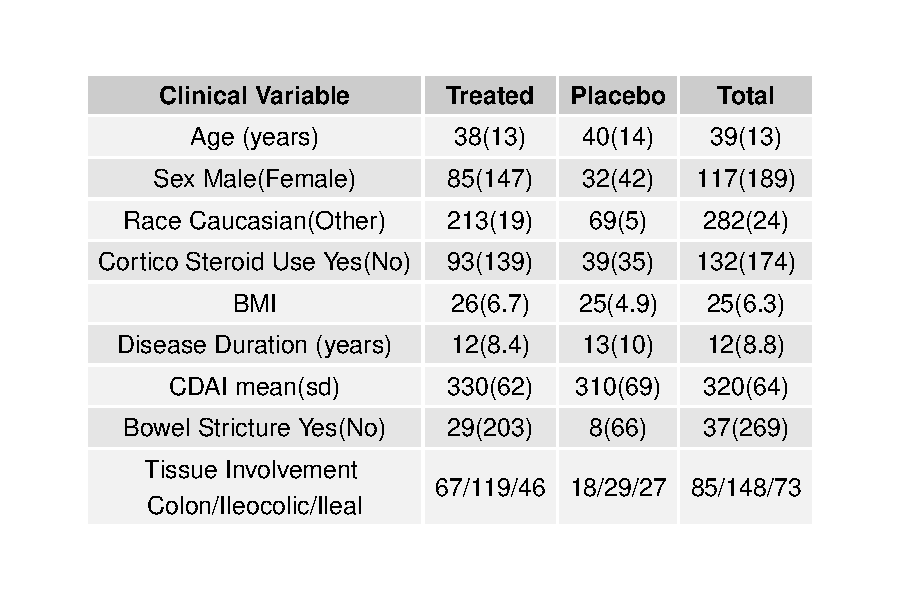
\includegraphics{tables/SupTable1_baseline_metadata.pdf}

\newpage

\textbf{Table 1: Diversity differences based on clinical metadata of
chort at baseline}

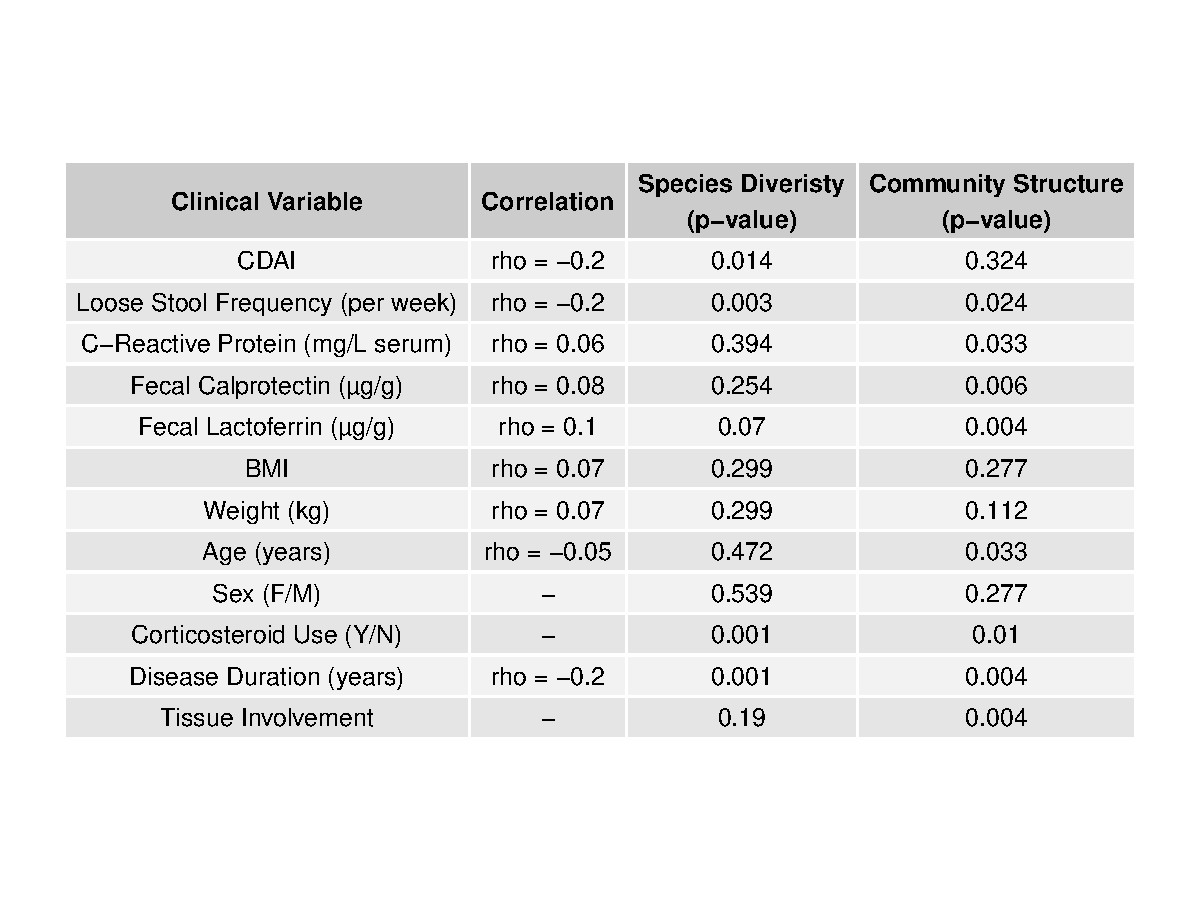
\includegraphics{tables/table1_cohortdiversity.pdf}

\newpage

\textbf{Table 2: Diversity differenced bases on Response/Remission in
treated subjects.}

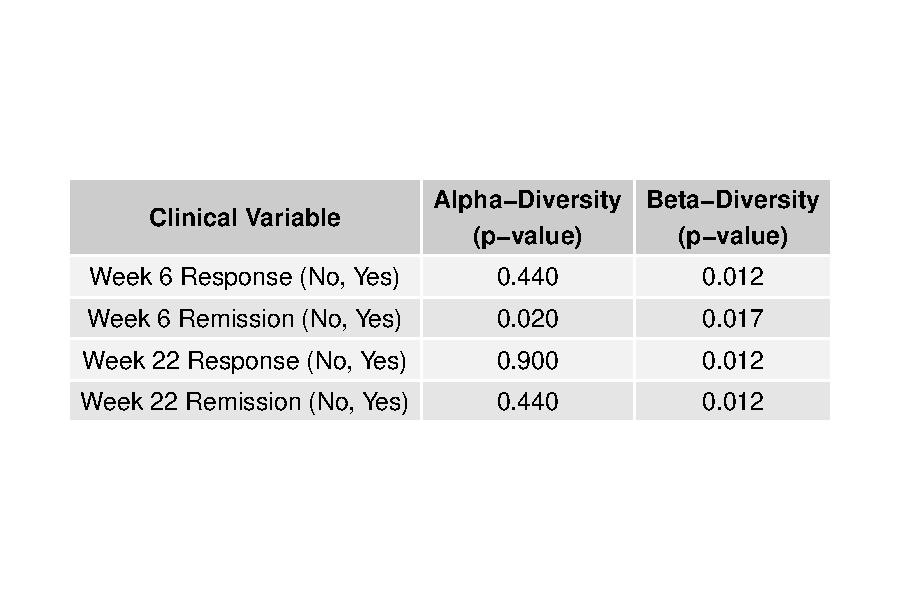
\includegraphics{tables/table2diversity.pdf}

\newpage

\textbf{Supplemental Table 2: Table of taxa that appear frequently in
predictive models at different response weeks, use baseline and
post-treat time points, also pooled}

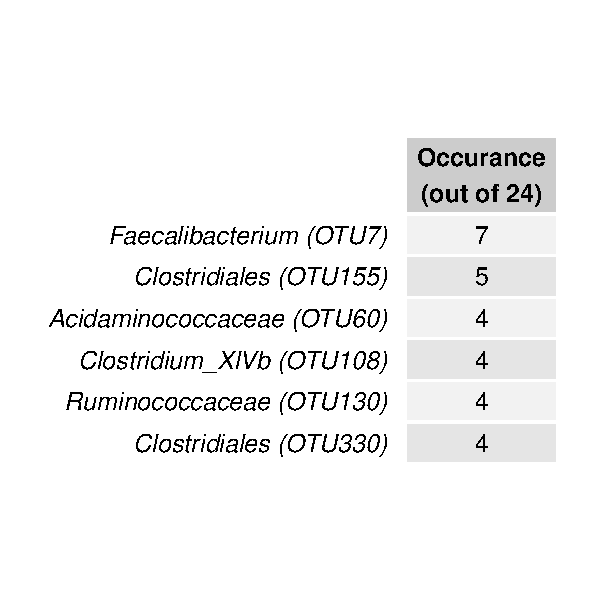
\includegraphics{tables/ST2_freqOTUs.pdf}

\newpage

\subsection{Figures}\label{figures}

\textbf{Figure 1: Prediction of RESPONSE/REMISSION in treated subjects
using all clinical metadata, baseline microbiome alone, and combined} A.
Response ROCs B. Response Model Performance vs.~reality C. Top
predictive taxa and abundance based on response D. REMISSION ROCs E.
REMISSION Model Performance vs.~reality F. Top predictive taxa and
abundance based on remission

\begin{figure}
\centering
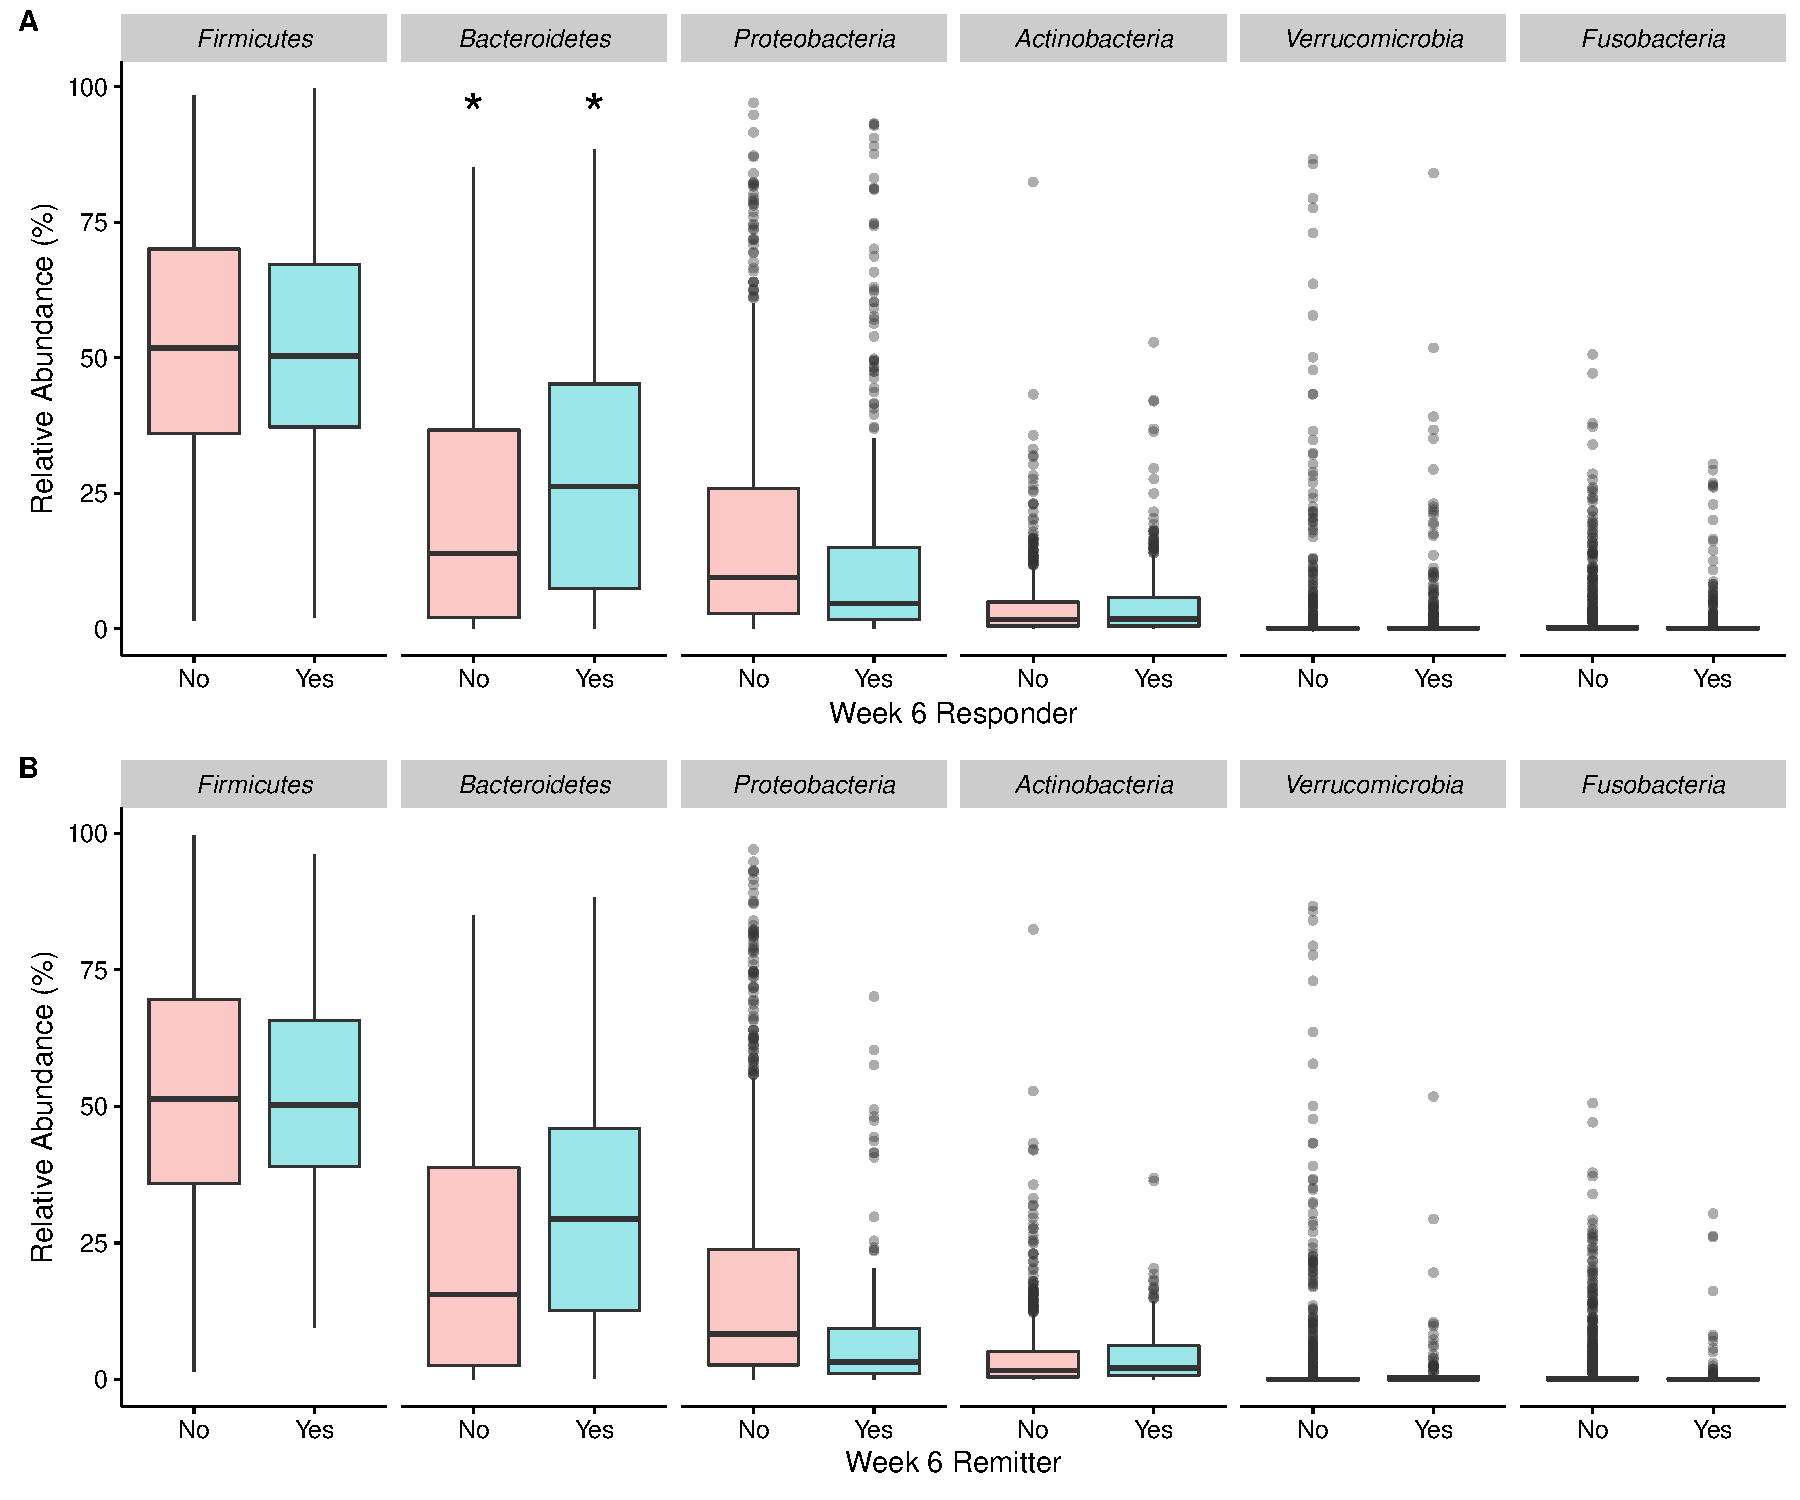
\includegraphics{figures/Figure1.tiff}
\caption{Prediction of RESPONSE/REMISSION in treated subjects using all
clinical metadata, baseline microbiome alone, and combined. A. Response
ROCs. B. Response Model Performance vs.~reality. C. Top predictive taxa
and abundance based on response. D. REMISSION ROCs. E. REMISSION Model
Performance vs.~reality. F. Top predictive taxa and abundance based on
remission}
\end{figure}

\newpage

\textbf{Figure 2: Lefse data supporting the abundance/importance data in
the predictive models} Abundance strip charts of differential taxa based
on A) response and B) remission.

\begin{figure}
\centering
\includegraphics{figures/Figure2LEfSe.tiff}
\caption{Figure 2: Lefse data supporting the abundance/importance data
in the predictive models. Abundance strip charts of differential taxa
based on A) response and B) remission.}
\end{figure}

\newpage

\textbf{Figure 3: Abundance of frequently predictive OTUs in responders
and remitters}

\begin{figure}
\centering
\includegraphics{figures/Figure3FreqOTUabund.tiff}
\caption{Abundance of frequently predictive OTUs in responders and
remitters}
\end{figure}

\newpage

\textbf{Supplemental Figure 1: Determining Week 6 disease status using
Week 6 samples}

\begin{figure}
\centering
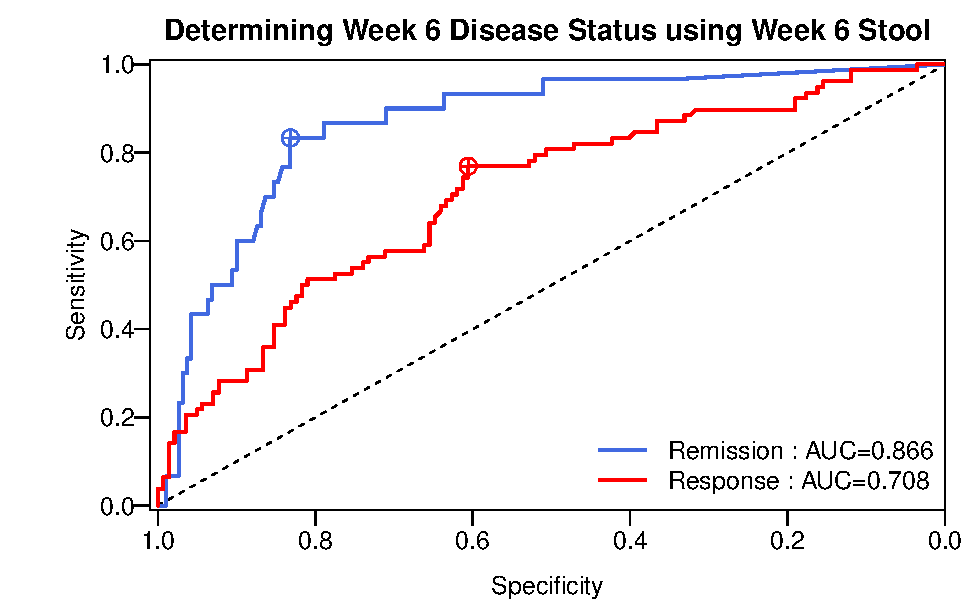
\includegraphics{figures/RSPwk6aucrf.tiff}
\caption{Supplemental Figure 1: Determining Week 6 disease status using
Week 6 samples}
\end{figure}

\newpage

\section*{References}\label{references}
\addcontentsline{toc}{section}{References}

\hypertarget{refs}{}
\hypertarget{ref-Ananthakrishnan_2015}{}
1. Ananthakrishnan AN. 2015. Epidemiology and risk factors for IBD.
Nature Reviews Gastroenterology \& Hepatology 12:205--217.

\hypertarget{ref-Floyd_2014}{}
2. Floyd DN, Langham S, Séverac HC, Levesque BG. 2014. The economic and
quality-of-life burden of crohn's disease in europe and the united
states, 2000 to 2013: A systematic review. Digestive Diseases and
Sciences 60:299--312.

\hypertarget{ref-Molodecky_2012}{}
3. Molodecky NA, Soon IS, Rabi DM, Ghali WA, Ferris M, Chernoff G,
Benchimol EI, Panaccione R, Ghosh S, Barkema HW, Kaplan GG. 2012.
Increasing incidence and prevalence of the inflammatory bowel diseases
with time, based on systematic review. Gastroenterology 142:46--54.e42.

\hypertarget{ref-Randall_2015}{}
4. Randall CW, Vizuete JA, Martinez N, Alvarez JJ, Garapati KV,
Malakouti M, Taboada CM. 2015. From historical perspectives to modern
therapy: A review of current and future biological treatments for
crohn's disease. Therapeutic Advances in Gastroenterology 8:143--159.

\hypertarget{ref-Boyapati_2015}{}
5. Boyapati R, Satsangi J, Ho GT. 2015. Pathogenesis of crohns disease.
F1000Prime Reports 7.

\hypertarget{ref-Wils_2016}{}
6. Wils P, Bouhnik Y, Michetti P, Flourie B, Brixi H, Bourrier A, Allez
M, Duclos B, Grimaud J-C, Buisson A, Amiot A, Fumery M, Roblin X,
Peyrin-Biroulet L, Filippi J, Bouguen G, Abitbol V, Coffin B, Simon M,
Laharie D, Pariente B. 2016. Subcutaneous ustekinumab provides clinical
benefit for two-thirds of patients with crohn's disease refractory to
antiTumor necrosis factor agents. Clinical Gastroenterology and
Hepatology 14:242--250.e2.

\hypertarget{ref-Colombel_2015}{}
7. Colombel J-F, Reinisch W, Mantzaris GJ, Kornbluth A, Rutgeerts P,
Tang KL, Oortwijn A, Bevelander GS, Cornillie FJ, Sandborn WJ. 2015.
Randomised clinical trial: Deep remission in biologic and
immunomodulator naïve patients with crohns disease - a SONIC post hoc
analysis. Alimentary Pharmacology \& Therapeutics 41:734--746.

\hypertarget{ref-Baert_2010}{}
8. Baert F, Moortgat L, Assche GV, Caenepeel P, Vergauwe P, Vos MD,
Stokkers P, Hommes D, Rutgeerts P, Vermeire S, D'Haens G. 2010. Mucosal
healing predicts sustained clinical remission in patients with
early-stage crohns disease. Gastroenterology 138:463--468.

\hypertarget{ref-Sandborn_2012}{}
9. Sandborn WJ, Gasink C, Gao L-L, Blank MA, Johanns J, Guzzo C, Sands
BE, Hanauer SB, Targan S, Rutgeerts P, Ghosh S, Villiers WJ de,
Panaccione R, Greenberg G, Schreiber S, Lichtiger S, Feagan BG. 2012.
Ustekinumab induction and maintenance therapy in refractory crohns
disease. New England Journal of Medicine 367:1519--1528.

\hypertarget{ref-Sandborn_2008}{}
10. Sandborn WJ, Feagan BG, Fedorak RN, Scherl E, Fleisher MR, Katz S,
Johanns J, Blank M, Rutgeerts P. 2008. A randomized trial of
ustekinumab, a human interleukin-12/23 monoclonal antibody, in patients
with moderate-to-severe crohns disease. Gastroenterology 135:1130--1141.

\hypertarget{ref-Kopylov_2014}{}
11. Kopylov U, Afif W, Cohen A, Bitton A, Wild G, Bessissow T, Wyse J,
Al-Taweel T, Szilagyi A, Seidman E. 2014. Subcutaneous ustekinumab for
the treatment of anti-TNF resistant crohns diseaseThe McGill experience.
Journal of Crohns and Colitis 8:1516--1522.


\end{document}
